
\chapter{Evaluation}
The evaluation has been divided into two different parts, one for each development method being evaluated. In 
\section{Native android} \label{android}
\subsection{Modularisation}
The android application has a lot of different responsibilities, apart from communicating with the native API and web application, it also has to contain the necessary activity threads to function as an application. A modularisation of the code into as small sections as possible has been the goal of the architecture being developed. The different responsibilities can be summarized as:

\begin{itemize}
\item Communication with the Android native API
\item Communication with the web application
\item Handling activity lifecycle
\item Starting activities for results (ex. the camera)
\end{itemize}


To conform to this modularisation, the architecture as figure \ref{caption-android-architecture} has been proposed. This divides the application into separate modules with a single responsibility, where the bridges responsibility is to handle communication between modules and add necessary logic for simple tasks such as casting of objects or performing calculations. 


\begin{figure}[ht!]
    \centering
    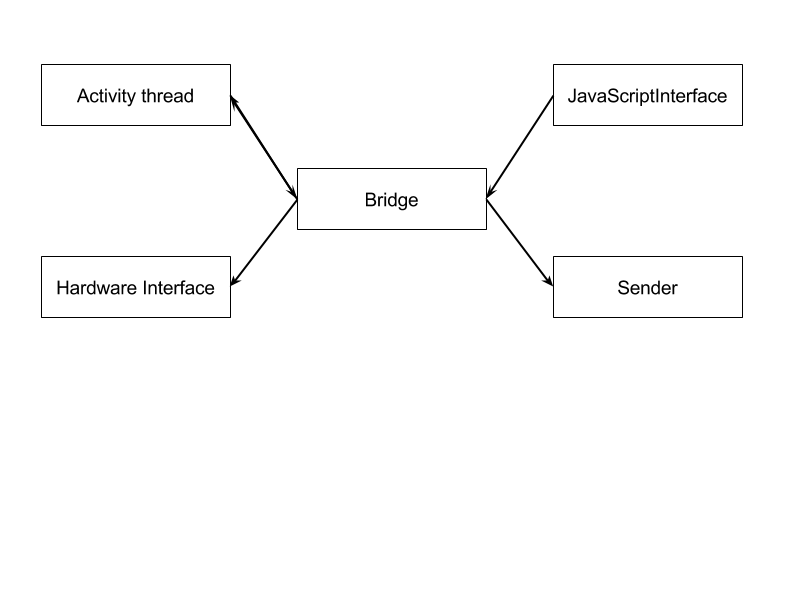
\includegraphics[width=120mm,natwidth=800,natheight=600]{./img/androidStructure.png}
    \caption{Architecture of the android application\label{caption-android-architecture}}
\end{figure}


(Add section describing function flow between java and javascript)

\begin{figure}[ht!]
    \centering
    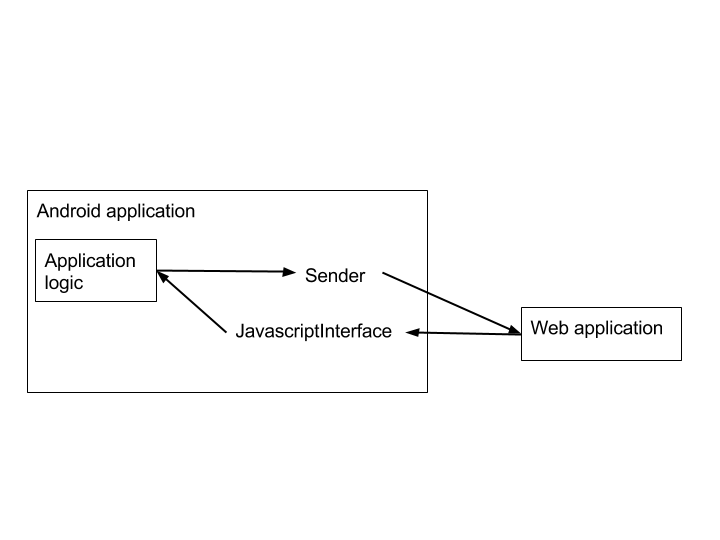
\includegraphics[width=120mm,natwidth=720,natheight=540]{./img/androidFlow.png}
    \caption{Function flow of the android application\label{caption-android-flow}}
\end{figure}

\subsection {Function calls between Java and JavaScript}
Calling javascript functions from Java is done using the function loadUrl on the WebView containing the web application. This was deducted to be an asynchronous method call, through practical tests in the development phase of this paper. 

(Add section containing example test here)

When calling java functions on the exposed javaScriptInterface object from javascript, the behavior of the function call is a bit more obscure. Due to the single-threaded nature of javascript, function calls are synchronous when called in a normal fashion.

(Add section containing example test here)

( However, by the usage of AJAX, the function calls may behave asynchronous on the web application side. Then the question arises, can two functions be executed in parallel on the android side, or is the execution of the jsInterface functions limited to being handled by a single thread. )<--Needs to be researched to stay here.

Utvärdering (Evaluation) bör beskriva den metod som används för att utvärdera din metod, inklusive experimentuppställning.
\section{Web application} 
\subsection{Results}
\subsubsection{Separating business logic from device specific logic}
An requirement on the web application is the ability to separate the business logic from device specific logic. This can be done with an adapter pattern. To set the right adapter a different method is used for Android and PhoneGap. The usage of this pattern ensures a natural way of modularising the code and separating all business logic from logic related to device-specific communication, the business logic is thus independent of the running device. 

\subsubsection{Encapsulating the web application in native Android application}
When encapsulating the web application when writing the mobile application in native Android code is done by the use of a WebView. When the web application is loaded in the native layer through a WebView an object is made available to the web application on which the web application can use to send messages to the native layer. Therefore checking if the web application is running within a WebView can be done by:
\begin{verbatim}
if(typeof Android !== 'undefined'){
 adapter = new AndroidAdapter()
}
\end{verbatim}
Where “Android” is the object made available to the web application by the native layer and can be used to invoke native functions.

\subsubsection{Encapsulating the web application in a PhoneGap application}
Here the same type of text as the chapter above shall be written


An overview of the recommended architecture for the web application can be seen below, where the internal structure of the mobile application is irrelevant. 

\begin{figure}[ht!]
    \centering
    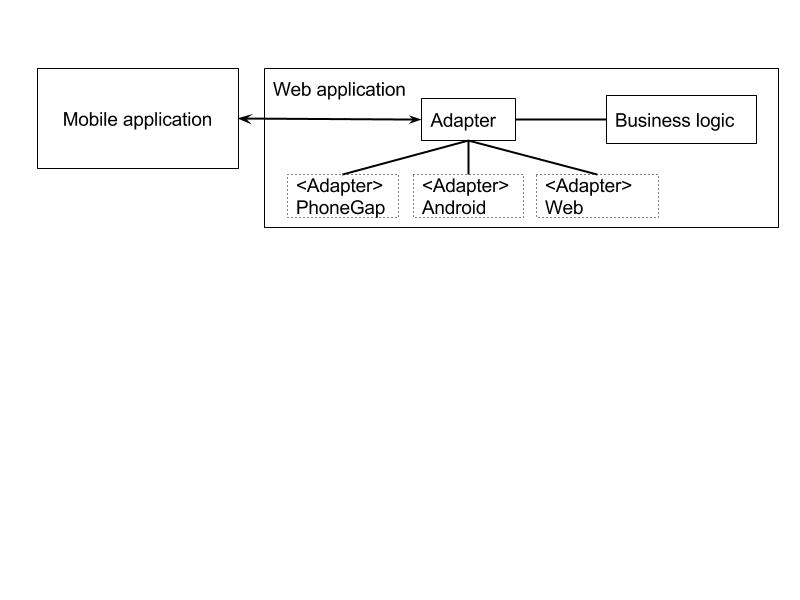
\includegraphics[width=140mm,natwidth=800,natheight=600]{./img/webAppFlow.jpg}
    \caption{Web application function calling flow \label{caption-web-flow}}
\end{figure}

\subsubsection{Communication between web application and mobile application}
(this chapter shall be rewritten)
Another functionality raising concerns regarding dependency is the communication between the web application and mobile application. The adapters dependency on the mobile application code is inevitable, unless communication can be made in a standardized way, and all devices expose methods conforming to an interface. The same thing goes for communication back to the web application, however in this case, the web application can expose a javascript function handling device callbacks, and as long as all devices are able to invoke javascripts in the web application, communication is independent apart from the name of the callback function. Ok that was not entirely true, in order for communication to be independent, all calls to the device must include the name of a callback function that will later be passed to the device callback function in the web application, which then relays callback data correctly. Also, the dependency on standardized callback data is still there, however this is a wanted behavior, as the data being sent back should be of the same type.

\section{PhoneGap}

\subsection{Communicatating between PhoneGap (native) layer and the web application}

\begin{figure}[ht!]
    \centering
    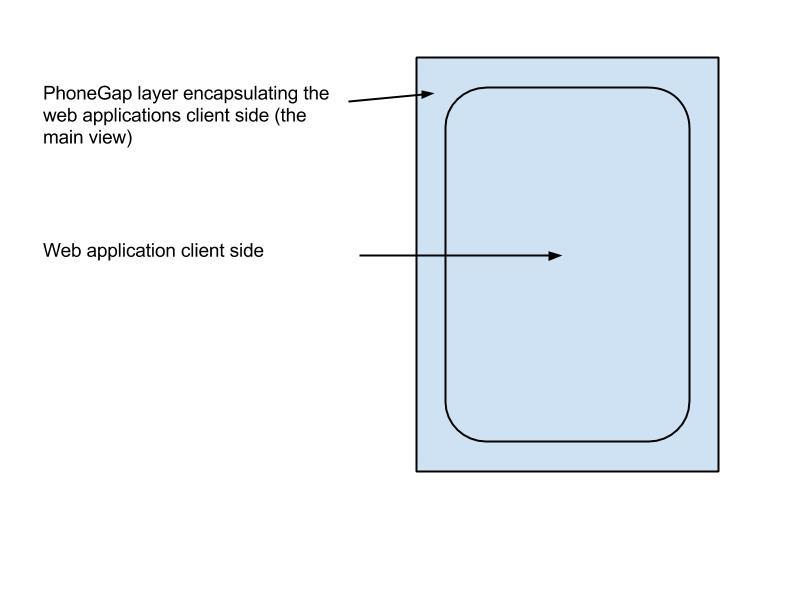
\includegraphics[width=120mm,natwidth=800,natheight=600]{./img/phonegap.jpg}
    \caption{The PhoneGap layer encapsulating the web application\label{overflow}}
\end{figure}


\subsubsection{Encupsulating the web application in an iFrame}
The remote web application is loaded in an iFrame, whilst PhoneGap logic is running in the main view (see picture). The default response header for a web page contains rules regarding same-origin policy, which disallows the webpage from being embedded in an iFrame on another web page, unless they have the same origin. The response header therefore needs to be modified, in order to allow web pages with other origins to load the webpage in an iFrame. 
This is done differently depending on the web development framework, in the framework Rails this can be done by: 

\begin{verbatim}
HomeController  < ApplicationController
  after_action :allow_iframe
  private
    def allow_iframe
      response.headers.except! 'X-Frame-Options'
     end
\end{verbatim}

Function calling from the web application is done by the use of postMessage on the parent window, the PhoneGap-layer listens to these messages by the use of an event listener. A request call from the web application is a message containing two key-value pairs: “type” and “callback”. The value of “type” specifies which native function the web application desires data from. The value of “callback” is used by the PhoneGap-layer when sending the data back to the web application. This is done with the predefined method deviceCallback on the adapter in the web application:

\begin{verbatim}
Adapter.deviceCallback(nativeData, calbackName);
\end{verbatim}

This way the PhoneGap layer only need to know in which format the data should be in, nothing else. 
\begin{figure}[ht!]
    \centering
    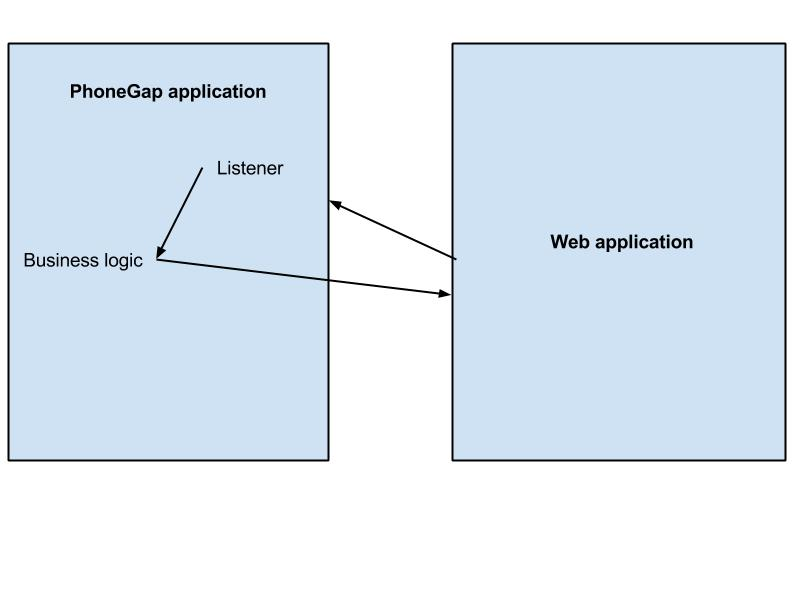
\includegraphics[width=120mm,natwidth=800,natheight=600]{./img/phoneGapFlow.jpg}
    \caption{PhoneGap function calling flow \label{caption-phonegap-flow}}
\end{figure}
\newline
The web application sends a message which is received by the listener in the PhoneGap application. The listener calls the function specified by the message, and passes on the callback to it. Upon completion the resulting data is passed to the web application, along with the callback, 

\subsubsection{Using polling in the PhoneGap plugin inAppBrowser}

inAppBrowser is a PhoneGap plugin which basically opens a browser “in the application”. By using this plugin to embed the remote web application, communication between the windows becomes different than when using an iFrame. Sending data from the PhoneGap-layer to the web application can be done by using the inAppBrowser function “executeScript”, which, in the inAppBrowser, executes the javascript passed as argument.

The communication back from the web application is more complicated. One example of how to do it is by the use of polling variables in the web application using executeScript. For further reading the following blog article: “Cross Window Communication With Cordova’s inAppBrowser” (http://blogs.telerik.com/appbuilder/posts/13-12-23/cross-window-communication-with-cordova\%27s-inappbrowser) by TJ VanToll is recommended. 

Other ways requires deeper technical web development knowledge. For more suggested methods read the support request https://issues.apache.org/jira/browse/CB-4897.

\subsubsection{Using a third party plugin}
PhoneGap supports custom plugins. This opens up the ability for companies to write their own plugins or make use of other third party plugins.

There is a PhoneGap plugin written by the corporation Wizcorp which claims it enables communication between the PhoneGap layer and web application. However despite extensive effort it never worked in this project. A ananswered support question (25/3-2015) can be seen at https://github.com/Wizcorp/phonegap-plugin-wizViewManager/issues/77. 

\subsection{Demo}
The demo code can be found at https://github.com/DavidNorrestam/pollux-phonegap. In the demo the communication between the PhoneGap layer and the web application is done by using an iFrame and postMessage, see chapter above. The most interesting files in the repository are found in:

\begin{description}
  \item[www/js/receiver.js] \hfill \\
    All the logic for receiving a message from the web application
  \item[www/js/device.js] \hfill \\
    Logic for some native functions and loading the web application
  \item[www/index.html] \hfill \\
    The html code for the mobile application view
\end{description}